% **************************************************
% Clean Thesis
% -- A LaTeX Style for Thesis Documents --
%
% Copyright (C) 2011-2013 Ricardo Langner
% **************************************************
%
% Readme:
% ----------------------------------------
% *** Clean, Simple, Elegant ***
% "Clean Thesis" is a LaTeX style for thesis documents, developed
% for my diplom thesis (Diplomarbeit). The style can be understood
% as my personal compromise - a typical clean looking scientific
% document combined and polished with minor beautifications.
%
% The design of this "Clean Thesis" style is inspired
% by user guide documents from Apple Inc.
%
% Note: If you are looking for an exact and correct style regarding
% typographic rules, please have a look at the "Classic Thesis Style"
% (see http://www.miede.de/index.php?page=classicthesis).
%
% *** Donation = Postcard ***
% Based on the idea of Andr\'e Miede: If you like the "Clean Thesis"
% style I would be very pleased about a donation in the form of a
% POSTCARD. You can find my address in the file Clean-Thesis.pdf.
% I am going to collect all postcards and exhibit them at the website
% I mentioned.
%
% *** Idea and Inspiration ***
% The idea of providing my customized style for thesis documents
% passed through my mind while writing my own thesis. Motivated and
% inspired by the superb "Classic Thesis Style"
% (see http://www.miede.de/index.php?page=classicthesis) by Andr\'e Miede
% (thanks to Andr\'e for doing a great job) I decided to collect all
% design and style related functionality in a separate LaTeX style and
% provide this style to other thesis writers.
%
%
% License Information:
% ----------------------------------------
% "Clean Thesis" is free software: you can redistribute it and/or modify
% it under the terms of the GNU General Public License as published by
% the Free Software Foundation, either version 3 of the License, or
% (at your option) any later version.
%
% "Clean Thesis" is distributed in the hope that it will be useful,
% but WITHOUT ANY WARRANTY; without even the implied warranty of
% MERCHANTABILITY or FITNESS FOR A PARTICULAR PURPOSE.  See the
% GNU General Public License for more details.
%
% You should have received a copy of the GNU General Public License
% along with this program.  If not, see <http://www.gnu.org/licenses/>.
% **************************************************


% **************************************************
% Document Class Definition
% **************************************************
\documentclass[%
	paper=A4,					% paper size --> A4 is default in Germany
	twoside=false,				% onesite or twoside printing
	openright,					% doublepage cleaning ends up right side
	parskip=full,				% spacing value / method for paragraphs
	chapterprefix=true,			% prefix for chapter marks
	11pt,						% font size
	headings=normal,			% size of headings
	bibliography=totoc,			% include bib in toc
	listof=totoc,				% include listof entries in toc
	titlepage=on,				% own page for each title page
	captions=tableabove,		% display table captions above the float env
	draft=false,				% value for draft version
]{scrreprt}%

% **************************************************
% Debug LaTeX Information
% **************************************************
%\listfiles

% **************************************************
% Information and Commands for Reuse
% **************************************************
\newcommand{\thesisTitle}{Barrierefreiheitsdatenbank}
\newcommand{\thesisSubtitle}{Untersuchung ob es eine Möglichkeit gibt Daten und Bilder auf mobilen Endgeräten offline zu Erfassen und bei bestehender Internetverbindung mit dem Server abzugleichen}
\newcommand{\thesisName}{Christian Schramm}
\newcommand{\thesisMatrikel}{s3001102}
\newcommand{\thesisSubject}{Belegarbeit Webprogrammierung}
\newcommand{\thesisDate}{April 8, 2014}
\newcommand{\thesisVersion}{0.0.1}

\newcommand{\thesisFirstReviewer}{Maksim Gudow}
% \newcommand{\thesisFirstReviewerUniversity}{\protect{webit! Gesellschaft für neue Medien mbH}}
\newcommand{\thesisFirstReviewerDepartment}{BERUFSAKADEMIE SACHSEN Staatliche Studienakademie Dresden}

% \newcommand{\thesisSecondReviewer}{Prof. Eberhardt Engelhardt}
% \newcommand{\thesisSecondReviewerUniversity}{\protect{BERUFSAKADEMIE SACHSEN
% Staatliche Studienakademie Dresden}}
% \newcommand{\thesisSecondReviewerDepartment}{Department of Clean Thesis Style}

% \newcommand{\thesisFirstSupervisor}{Jane Doe}
% \newcommand{\thesisSecondSupervisor}{John Smith}

\newcommand{\thesisUniversity}{\protect{BERUFSAKADEMIE SACHSEN Staatliche Studienakademie Dresden}}
% \newcommand{\thesisUniversityDepartment}{}
% \newcommand{\thesisUniversityInstitute}{Institut for Clean Thesis Dev}
% \newcommand{\thesisUniversityGroup}{Clean Thesis Group (CTG)}
\newcommand{\thesisUniversityCity}{Dresden}
\newcommand{\thesisUniversityStreetAddress}{Hans-Grundig-Straße 25}
\newcommand{\thesisUniversityPostalCode}{01307}

% **************************************************
% Load and Configure Packages
% **************************************************
\usepackage[utf8]{inputenc}		% defines file's character encoding
\usepackage[ngerman]{babel} % babel system, adjust the language of the content
\usepackage[printonlyused,footnote,nohyperlinks]{acronym}

\usepackage{scrhack}

\usepackage[					% clean thesis style
	figuresep=colon,%
	sansserif=false,%
	hangfigurecaption=false,%
	hangsection=true,%
	hangsubsection=true,%
	colorize=full,%
	colortheme=bluemagenta,%
]{cleanthesis}

\hypersetup{					% setup the hyperref-package options
	pdftitle={\thesisTitle},	% 	- title (PDF meta)
	pdfsubject={\thesisSubject},% 	- subject (PDF meta)
	pdfauthor={\thesisName},	% 	- author (PDF meta)
	plainpages=false,			% 	-
	colorlinks=false,			% 	- colorize links?
	pdfborder={0 0 0},			% 	-
	breaklinks=true,			% 	- allow line break inside links
	bookmarksnumbered=true,		%
	bookmarksopen=true			%
}

% **************************************************
% Document CONTENT
% **************************************************
\begin{document}

% --------------------------
% rename document parts
% --------------------------
\renewcaptionname{ngerman}{\figurename}{Abb.}
\renewcaptionname{ngerman}{\tablename}{Tab.}
% \renewcaptionname{english}{\figurename}{Fig.}
% \renewcaptionname{english}{\tablename}{Tab.}

% --------------------------
% Front matter
% --------------------------
\pagenumbering{roman}			% roman page numbing (invisible for empty page style)
\pagestyle{empty}				% no header or footers
% !TEX root = ../thesis-example.tex
%
% ------------------------------------  --> cover title page
\begin{titlepage}
	\pdfbookmark[0]{Cover}{Cover}
	\flushright
	\hfill
	\vfill
	{\LARGE\thesisTitle} \par
	\rule[5pt]{\textwidth}{.4pt} \par
	{\Large\thesisName}
	\vfill
	\textit{\large\thesisDate} \\
	Version: \thesisVersion
\end{titlepage}


% ------------------------------------  --> main title page
\begin{titlepage}
	\pdfbookmark[0]{Titlepage}{Titlepage}
	\tgherosfont
	\centering

	{
\includegraphics[width=2cm]{Bilder/ba_logo} \\[2mm]}
	{\Large \thesisUniversity \\[4mm]}
	% \textsf{\thesisUniversityDepartment} \\
	% \textsf{\thesisUniversityInstitute} \\
	% \textsf{\thesisUniversityGroup} \\

	\vfill
	{\large \thesisSubject} \\[5mm]
	{\LARGE \color{ctcolormain}\textbf{\thesisTitle} \\[10mm]}
	{\Large \thesisName} \\

	\vfill
	\begin{minipage}[t]{.27\textwidth}
		\raggedleft
		% \textit{Erstgutachter}
		\textit{Gutachter}
	\end{minipage}
	\hspace*{15pt}
	\begin{minipage}[t]{.65\textwidth}
		{\Large \thesisFirstReviewer} \\
	  	{\small \thesisFirstReviewerDepartment} \\[-1mm]
		% {\small \thesisFirstReviewerUniversity}
	\end{minipage} \\[5mm]
	% \begin{minipage}[t]{.27\textwidth}
	% 	\raggedleft
	% 	\textit{Zweitgutachter}
	% \end{minipage}
	\hspace*{15pt}
	% \begin{minipage}[t]{.65\textwidth}
	% 	{\Large \thesisSecondReviewer} \\
	%   	{\small \thesisSecondReviewerDepartment} \\[-1mm]
	% 	{\small \thesisSecondReviewerUniversity}
	% \end{minipage} \\[10mm]
	% \begin{minipage}[t]{.27\textwidth}
	% 	\raggedleft
	% 	\textit{Supervisors}
	% \end{minipage}
	% \hspace*{15pt}
	% \begin{minipage}[t]{.65\textwidth}
	% 	\thesisFirstSupervisor\ and \thesisSecondSupervisor
	% \end{minipage} \\[10mm]

	\thesisDate \\

\end{titlepage}


% ------------------------------------  --> lower title back for single page layout
\hfill
\vfill
\small
\textbf{\thesisName} \\
\textit{\thesisTitle} \\
\thesisSubject, \thesisDate \\
Gutachter: \thesisFirstReviewer\\
% und \thesisSecondReviewer \\
% Supervisors: \thesisFirstSupervisor\ and \thesisSecondSupervisor \\[1.5em]
\textbf{\thesisUniversity} \\
% \textit{\thesisUniversityGroup} \\
% \thesisUniversityInstitute \\
% \thesisUniversityDepartment \\
\thesisUniversityStreetAddress \\
\thesisUniversityPostalCode\ \thesisUniversityCity
		% INCLUDE: all titlepages
\cleardoublepage

% \pagestyle{plain}				% display just page numbers
% % !TEX root = Clean-Thesis.tex
%
\pdfbookmark[0]{Abstract}{Abstract}
\chapter*{Abstract}
\label{sec:abstract}
\vspace*{-10mm}

\blindtext

\vspace*{20mm}

{\usekomafont{chapter}Abstract (different language)}\label{sec:abstract-diff} \\

\blindtext
		% INCLUDE: the abstracts (english and german)
% \cleardoublepage
%
% % !TEX root = ../thesis-example.tex
%
\pdfbookmark[0]{Acknowledgement}{Acknowledgement}
\chapter*{Acknowledgement}
\label{sec:acknowledgement}
\vspace*{-10mm}

\Blindtext[2][2]
 % INCLUDE: acknowledgement
% \cleardoublepage
%
\setcounter{tocdepth}{2}		% define depth of toc
\tableofcontents				% display table of contents
\cleardoublepage

% --------------------------
% Body matter
% --------------------------
\pagenumbering{arabic}			% arabic page numbering
\setcounter{page}{1}			% set page counter
\pagestyle{maincontentstyle} 	% fancy header and footer

% !TEX root = ../thesis-example.tex
%
\chapter{Einleitung}
\label{sec:Einleitung}

\cleanchapterquote{There are two ways of constructing a software design: One way is to make it so simple that there are obviously no deficiencies, and the other way is to make it so complicated that there are no obvious deficiencies. The first method is far more difficult.}{C.A.R. Hoare}{(British computer scientist, winner of the 1980 Turing Award)}

Das Thema Barrierefreiheit betrifft einen jährlich zunehmenden größer werdenden Teil der Bevölkerung. Im Jahr 2011 gab es mit knapp 7,3 Millionen schwerbehinderten Menschen rund 2,6\% mehr als noch im Jahr 2009.\cite[]{WEB:DESTATIS:2014} Dabei leiden zweidrittel der schwerbehinderten Menschen unter körperlichen Behinderungen, welche je nach Grad und Art der Behinderung zu sehr starken Einschränkungen im Alltag führen können.

Im Bereich des öffentlichen Lebens wird sehr viel dafür getan, um z.B. die Zugänge zu öffentlichen Einrichtungen wie Museen, Ämtern oder öffentlichen Verkehrsmitteln zu erleichtern. In der Verordnung DIN 18040 Barrierefreies Bauen sind grundlegende Anforderungen an öffentlich zugängliche Gebäude beschrieben. Die Einführung dieser Verordnung bzw. der einzelnen Punkte in die Technischen Baubestimmungen obliegt jedoch den einzelnen Bundesländern.\cite[]{WEB:DIN18040:2010}

Um erfassen zu können welche Einrichtungen die behindertengerechten Anforderungen erfüllen, wurde von der Thüringer Tourismus GmbH in Zusammenarbeit mit dem Dresdner Unternehmen webit! Gesellschaft für neue Medien mbH das Konzept der Barrierefreiheitsdatenbank entwickelt. Sie ermöglicht es alle Daten über eine Einrichtung zu erfassen. Dazu zählen z.B. Zugänge, Treppen, Liftanlagen und vieles mehr. Alle Daten die von Mitarbeitern des Unternehmens erfasst werden, kommen in einer Datenbank zusammen und sollen dabei helfen behinderten Menschen bei der Planung ihres Urlaubs oder von Ausflügen zu unterstützen.

\section{Motivation}
\label{sec:motivation:mot}

Die Überlegung zu dieser Arbeit kam durch die Erfassung der ersten öffentlich begehbaren Einrichtungen. Um zum derzeitigen Zeitpunkt Daten erfassen zu können, wird eine Internetverbindung benötigt. Diese kann aber bei vielen Einrichtungen, wie z.B. Kellergewölben, Museen oder Schlössern nicht gewährleistet werden. Dadurch entstand der Wunsch die Daten unabhängig von einer Internetverbindung einpflegen zu können. Die aufgenommenen Bilder und Informationen zu den baulichen Gegebenheiten sollen dann mit den vorhandenen Daten auf dem Server abgeglichen werden und gegebenenfalls auf dem Client, als auch auf dem Server ergänzt werden.

\section{Zielstellung und Abgrenzung der Arbeit}
\label{sec:goal:goal}

Smartphones und Tablets gehören mittlerweile zum Standard der mobilen Kommunikation. Mit diesen kleinen \"Alleskönnern\" kann man Fotos aufnehmen, im Internet surfen, Dokumente erfassen und vieles mehr, was noch vor ein paar Jahren nur von Desktoprechnern denkbar gewesen wäre. Das macht die heutige Datenerfassung sehr viel flexibler als noch vor ein paar Jahren.

Ziel der Arbeit ist es eine Möglichkeit zu finden, Daten die mit mobilen Endgeräten erfasst werden mit den Daten auf einem Server zu synchronisieren.  Dabei soll sowohl die Datenbank betrachtet werden, als auch Bilddateien. Als Ausgangspunkt dienen die Vor- und Nachteile die es bei nativen Apps, Web Apps und einer Hybrid App Variante gibt und wie sich das auf eine Synchronisation der Daten auswirkt.

In dieser Arbeit wird keine native App und auch keine Webapp programmiert, sondern nur Überlegungen zur Umsetzung einer erfolgreichen Synchronisation getroffen, die dann eine Entscheidung über die Wahl der mobilen Variante der Barrierefreiheitsdatenbank beeinflussen könnte.

\section{Untersuchungsgegenstand}
\label{sec:investigation:inv}

Um die nachfolgende Forschungsfrage wiederlegen oder bestätigen zu können, werde ich mir unterschiedliche Methoden der Datensynchronisation anschauen und die Vor- und Nachteile miteinander vergleichen und für das Kundenprojekt einen Lösungsansatz zu finden.

\subsection{Forschungsfrage}
\label{subsec:problem:prob}

Nach Betrachtung der Zielstellung ergab sich eine Forschungsfrage, die am Ende der Arbeit beantwortet werden soll.

\begin{quote}
	\textbf {Gibt es eine Möglichkeit alle Daten die mit mobilen Endgeräten offline erfasst werden, bei bestehender Internetverbindung mit dem Server abzugleichen?}
\end{quote}

\cleardoublepage

\subsection{Hypothesen}
\label{subsec:hypothesis:hypo}

Daraus ergaben sich folgende Hypothesen, welche sich bei der Untersuchung der Methoden als richtig oder falsch herausstellten.

\textbf {1. Hypothese}

Es lassen sich alle mit einem mobilen Endgerät erfassten Daten uneingeschränkt per Internet mit dem Server synchronisieren.

\textbf {2. Hypothese}

Die Entwicklung einer nativen App ist die beste Lösung für die Nutzung der Hardwarefunktionen und des Speicherbedarfs der Kombination aus Datenbank und Bildern.

\textbf {3. Hypothese}

Die Umsetzung einer Web App bietet sich aufgrund der bestehenden Website an. Dadurch verringern sich Aufwand und Kosten, ohne Einschränkung der Funktionen.
 % INCLUDE: introduction
% !TEX root = ../thesis-example.tex
%
\chapter{Theorie/Begriffsbestimmung}
\label{sec:theorie:Theorie}

\cleanchapterquote{Most good programmers do programming not because they expect to get paid or get adulation by the public, but because it is fun to program.}{Linus Torvalds}{(Finnish American, software engineer and hacker)}

Um das allgemeine Verständnis zu gewährleisten müssen noch einige wichtige Begriffe geklärt werden, die die Grundlage für die folgende Untersuchung bilden.

Die Entscheidung, welche der mobilen Variante man für die Umsetzung verwendet ist abhängig von den jeweiligen Eigenschaften. Auf wieviel Speicher darf die App zugreifen, welche Handyfunktionen werden benötigt und lässt sich feststellen wann eine Internetverbindung besteht und lassen sich davon abhängig die Daten mit dem Server abgleichen.

\section{Native Apps}
\label{sec:intro:native}

Die Nativen Apps werden speziell für das jeweilige Betriebssystem entwickelt z.B. iOS oder Android. Diese laufen dann auch ausschließlich auf iOS Geräten wie dem iPhone und dem iPad, oder Android Geräten wie dem Samsung Galaxy S4.\cite[]{WEB:APPEV:2014}

Dadurch stellt man eine optimale Nutzung der Ressourcen und einheitlich funktionierende Hardwareschnittstellen sicher.\cite[]{WEB:APPEV:2014}

\subsection{Vorteile}
\label{sec:native:pros}

\begin{itemize}

	\item Native Apps nutzen die Leistung des Betriebssystems und des verwendeten Gerätes voll aus, da sie speziell für das Betriebssystem angepasst sind. Dadurch lassen sich sehr gut komplexere und rechenintensivere Apps umsetzen.\cite[]{WEB:APPEV:2014}

	\item Durch die Installation der Apps auf dem Endgerät, können Hardwarefunktionen wie Kamera, Beschleunigungssensor oder \ac{GPS} benutzt werden. Das ist in der Regel nur nativen Apps vorbehalten.\cite[]{WEB:APPEV:2014}

	\item Daten können auf dem Endgerät in beliebiger Menge gespeichert werden.\cite[]{WEB:APPEV:2014}

	\item Da Native Apps über einen Appstore vertrieben werden, werden diese öfter gekauft, wenn Sie über gute Bewertungen verfügen.\cite[]{WEB:APPEV:2014}

	\item Die App lässt sich sehr einfach über den Appstore installieren und es wird automatisch ein Icon zum Starten angelegt.\cite[]{WEB:APPEV:2014}

	\item Der Vertriebsaufwand ist sehr gering, da die Appstores verbreitete Bezugsquellen für Native Apps sind. Ist die App erfolgreich, kann man sich in den Top-Listen der App Stores wiederfinden und dadurch sehr hohe Downloadzahlen erreichen.\cite[]{WEB:APPEV:2014}

\end{itemize}

\subsection{Nachteile}
\label{sec:native:cons}

\begin{itemize}

	\item Ein großer Nachteil ist der erforderliche Entwicklungsaufwand, wenn man die App in allen Appstores anbieten möchte. Dafür muss man die App an die jeweiligen Gegebenheiten des Betriebssystems optimieren.\cite[]{WEB:APPEV:2014}

	\item Es entstehen zusätzliche Kosten um die App für den entsprechenden entwicklen und anbieten zu können.

\end{itemize}

\section{Webapps}
\label{sec:intro:webapp}

Die sogenannten Webapps sind im eigentlichen Sinne speziell programmierte \ac{HTML5} Websites, die erkennen auf welchem Endgerät sie aufgerufen werden und optimieren den Inhalt entsprechend. Somit kann quasi jedes mobile Endgerät, dass über einen Webbrowser verfügt, die App nutzen.

\subsection{Vorteile}
\label{sec:webapp:pros}

\begin{itemize}

	\item Web Apps sind quasi unabhängig vom Betriebssystem und funktionieren auf allen Smartphones. Dadurch erreicht man mehr potentielle Nutzer, bei gleichzeitig geringeren Kosten.\cite[]{WEB:APPEV:2014}

	\item In der Regel kommt man mit der Entwicklung einer Web App günstiger, als mit der Entwicklung einer nativen App für nur ein Betriebssystem.\cite[]{WEB:APPEV:2014}

	\item Durch die Verwendung von HTML5 wird auch die Offline-Speicherung von Daten ermöglicht. Somit kann man auch ohne permanente Internetverbindung die einmal geladene Web App nutzen.\cite[]{WEB:APPEV:2014}

	\item Über Onlinesuchmaschinen wie z.B. Google können Web Apps ohne großen Aufwand gefunden werden und lassen sich auch ohne Installation direkt nutzen. Speichert man diese als Lesezeichen, lässt sie sich genau wie eine Native App vom Startbildschirm aus starten.\cite[]{WEB:APPEV:2014}

	\item Die Veröffentlich und Aktualisierung erfolgt in Sekundenschnelle, da sie im Gegensatz zu Nativen Apps keinen Zulassungsprozess durchlaufen müssen.\cite[]{WEB:APPEV:2014}

	\item Vertreibt man die App selbst, entfällt die Provision von überlicherweise 30\% an den Betreiber des App Stores.\cite[]{WEB:APPEV:2014}

	\item Hat man vor die irgendwann die Vorteile einer nativen App zu nutzen und beachtet das bei der Programmierung der Web App, lässt sich diese leicht und kostengünstig in eine Native App umwandeln.\cite[]{WEB:APPEV:2014}

\end{itemize}

\subsection{Nachteile}
\label{sec:webapp:cons}

\begin{itemize}

	\item Die meisten Hardwarefunktionen der mobilen Geräte lassen sich garnicht oder nur mit spezieller Zustimmung des Nutzers verwenden.\cite[]{WEB:APPEV:2014}

	\item Komplexe Berechnungen wie z.B. 3D Darstellungen, Verschlüsselung oder Bildbearbeitungen sind mit einer Web App nicht möglich.\cite[]{WEB:APPEV:2014}

	\item Benötigt die App mehr als 10MB an Datenmaterial auf dem Endgerät ist von einer Entwicklung als reine Web App abzusehen.\cite[]{WEB:APPEV:2014}

	\item Geschäftsmodelle die auf In-App-Käufe oder einen App Store aufbauen, funktionieren zusammen mit der Web App nicht.\cite[]{WEB:APPEV:2014}

\end{itemize}

\section{Hybridapps}
\label{sec:intro:hybrid}

Hybridapps sollen die Vorteile der Web App Entwicklung und der Entwicklung von nativen Apps in sich vereinen. Dabei setzen die Entwickler auf eine große Anzahl von Frameworks. PhoneGap, Corona oder Appelerator Titanium sind Beispiele dafür, mit deren Hilfe man Web Apps in eine native App umwandeln kann.

Für Einige mag die Entwicklung einer Hybridapp als \"Allheilmittel\" klingen, jedoch gibt es auch hier Vor- und Nachteile.\cite[]{WEB:APPEV:2014}

\subsection{Vorteile}
\label{sec:hybrid:pros}

\begin{itemize}

	\item Durch die Verwendung einer Hybrid App lässt sich eine Cross Browser Web App erstellen, die in allen modernen Browsern läuft.\cite[]{WEB:APPEV:2014}

	\item Da eine Web App mittels Frameworks für verschiedene Betriebssysteme umgewandelt werden kann, erspart man sich die eigenständige Entwicklung für jedes einzelne Betriebssystem. Es bleiben im schlimmsten Fall nur Betriebssystemspezifische Feinheiten, die noch angepasst werden müssen.\cite[]{WEB:APPEV:2014}

	\item Mit Javascript lassen sich viele Hardwarefunktionen der Endgeräte nutzen, auf die man bei einer Web App nicht zugreifen konnte.\cite[]{WEB:APPEV:2014}

	\item Der Verkauf einer Hybrid App kann wieder über den jeweiligen App Store erfolgen.\cite[]{WEB:APPEV:2014}

\end{itemize}

\subsection{Nachteile}
\label{sec:hybrid:cons}

\begin{itemize}

	\item Ein großer Nachteil der Hybridapps kann entstehen, wenn man sehr rechenintensive Anwendungen verwendet. Dadurch können Hybrid Apps sehr schnell an das Leistungsmaximum herranreichen und träge reagieren. Das ist sehr stark von dem verwendeten Framwork abhängig und ein Nachteil der in Zukunft durch merklich effizienter werdende Frameworks behoben werden kann.\cite[]{WEB:APPEV:2014}

	\item Die Progammierung einer Hybrid App könnte mit zunehmendem Komplexitätsgrad sehr aufwendig werden und eine Umsetzung mittels nativer App empfehlenswerter machen.\cite[]{WEB:APPEV:2014}

\end{itemize}

\section{Wahl der Appvariante}
\label{sec:intro:Appvariante}

Die Wahl der Appvariante ist nicht allein abhängig von den Vor- und Nachteilen der Varianten. Hierfür muss man auch die bestehende Website betrachten und die Umsetzungsaufwände gegeneinander abwägen.

Ein nicht zu unterschätzender Vorteil der Website ist die bereits responsive Umsetzung. (Abb.\ref{Barrierefreidatenbank}-\ref{Websitemobil}) Dadurch passt sich der dargestellte Inhalt an das Endgerät an, wodurch optimale Darstellung auch auf mobilen Geräten gewährleistet wird. Es können somit bereits neue Daten mobil erfasst werden.

\begin{figure}[htb]
	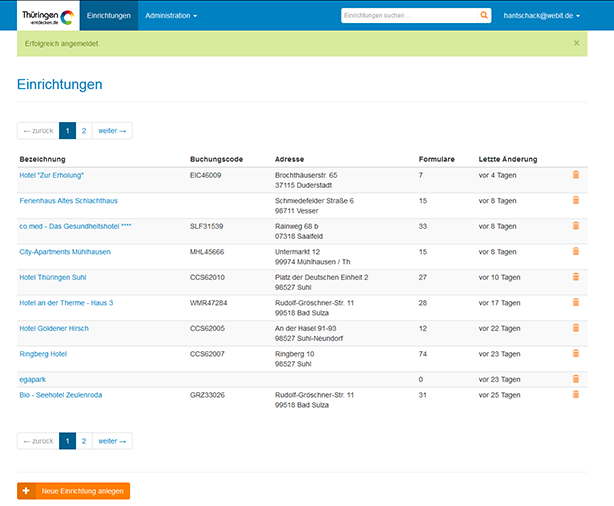
\includegraphics[width=\textwidth]{Bilder/Barrierefreidatenbank}
	\caption{Barrierefreiheitsdatenbank}
	\label{Barrierefreidatenbank}
\end{figure}

\begin{figure}[htb]
	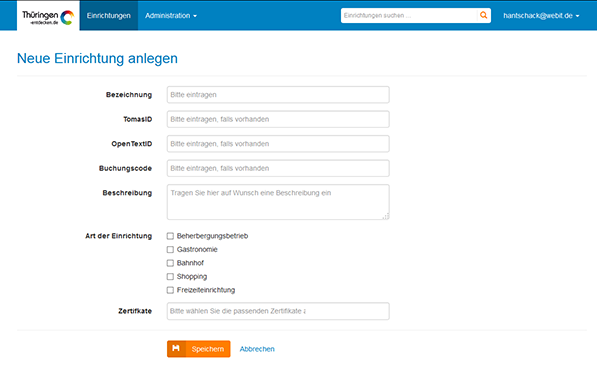
\includegraphics[width=\textwidth]{Bilder/Datenerfassung}
	\caption{Datenerfassung}
	\label{Datenerfassung}
\end{figure}

\begin{figure}[htb]
	\begin{tabular}{l r}
		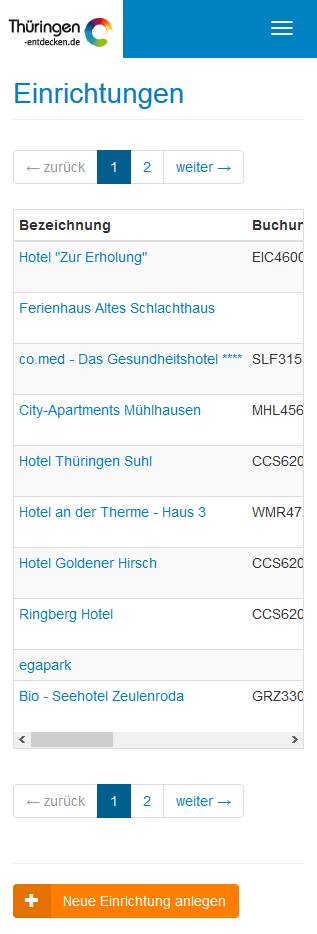
\includegraphics[width=0.49\textwidth]{Bilder/Barrierefreidatenbank-mobil}
		&
		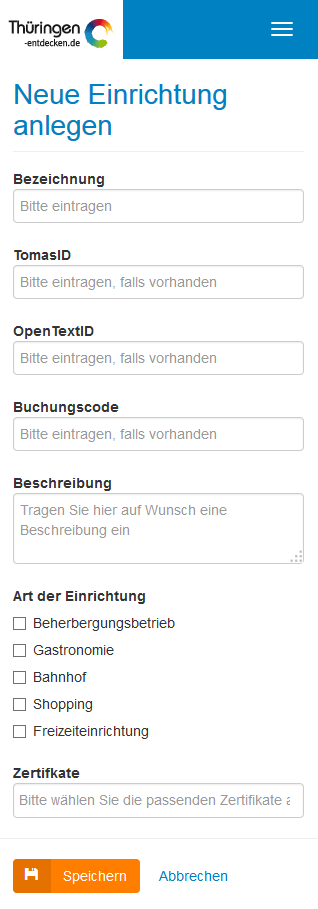
\includegraphics[width=0.49\textwidth]{Bilder/Datenerfassung-mobil}
	\end{tabular}
	\caption{Barrierefreiheitsdatenbank mobil}
	\label{Websitemobil}
\end{figure}

\cleardoublepage

Nach Betrachtung der Vor- und Nachteile der App Varianten und der bestehenden Website, schließe ich die Umsetzung einer reinen nativen App aus. Der Umsetzungsaufwand und die entstehenden Kosten wären unangemessen hoch im Vergleich zu den daraus entstehenden Vorteilen.

Da eine Web App auf \ac{HTML5} aufbaut und die Website sich bereits teilweise an das Endgerät anpasst, baut die Untersuchung im auf eine Umsetzung als Web App auf. Daher wird bei der Synchronisation auf \ac{HTML5} und Javascript gesetzt. % INCLUDE: Grundlagen
% !TEX root = ../thesis-example.tex
%
\chapter{Synchronisation}
\label{sec:Synchronisation}

\cleanchapterquote{The most important property of a program is whether it accomplishes the intention of its user.}{C.A.R. Hoare}{(British computer scientist, winner of the 1980 Turing Award)}

Synchronisation beschreibt den Datenaustausch zwischen einem Sender und einem Empfänger. Dabei werden die Daten in Blöcke aufgeteilt und in einen Übertragungsrahmen eingepasst. Um die Daten aneinander anzugleichen muss dabei festgestellt werden, welches Endgerät welche Daten besitzt und kontrolliert ob das andere Gerät diese Daten zu seinen besitzen will.

Besitzen beide Endgeräte dieselben Daten, z.B. in unterschiedlichen Versionen, kann definiert werden, wie mit den Änderungen umgegangen wird.\cite[]{WEB:SYNCML:2014}

Durch die Begrenzung des lokalen Gerätespeichers würde ich die Synchronisation auf 2 seperaten Wegen durchführen. Im ersten Teil die Datenbank und als Zweites alle Anhänge, wie z.B. Bilder oder Dokumente. So kann das Problem der Speicherbegrenzung bei Webapps umgangen werden.

\section{Datenbanksynchronisation am Bsp. WebSqlSync}
\label{sec:dbsync}

WebSqlSync ist eine Javascript Bibliothek zur automatischen Synchronisation einer lokalen WebSql Datenbank mit dem Server. Die Synchronisation kann dabei in beide Richtungen erfolgen und arbeitet auf dem Prinzip der inkrementellen Synchronisation, was bedeutet dass nur erforderliche Daten übertragen werden.

WebSqlSync funktioniert auch ohne Internetverbindung. Alle Änderungen der Daten werden dabei verfolgt und mit dem Server abgeglichen, sobald wieder eine Internetverbindung besteht. Es wird auch die Änderung auf mehreren Geräten unterstützt.

Die Unterstützung von webapp und der phonegap app für mobile Betriebssysteme wie z.B. iOS und Android ermöglicht eine einfache Integration ohne den Programmcode anpassen zu müssen.\cite[]{WEB:WEBSQLSYNC:2014}

\cleardoublepage

\textbf{Installation und Initialisierung}

Um WebSqlSync nutzen zu können, muss nur die Datei webSqlSync.js im \ac{HTML} des Projekts hinzugefügt werden.

\lstset{language=html}
\lstinline$<script src="lib/webSqlSync.js" type="application/x-javascript" charset="utf-8"></script>$

Wird die Bibliothek aufgerufen, werden automatisch 2 Datenbanktabellen erstellt, falls diese nicht bereits von einem vorherigen Aufruf existieren. Die erste Tabelle \textbf{\lstinline$new_elem$} speichert alle neuen bzw. geänderten Elemente und die zweite Tabelle \textbf{\lstinline$sync_info$} das Datum der letzten Synchronisation.

Zusätzlich werden sogenannte SQLite Auslöser erstellt, die überwachen ob Änderungen per \textbf{\lstinline$INSERT$} oder \textbf{\lstinline$UPDATE$} an den Tabellen vorgenommen wird. SQLite ist eine einfache Datenbankbibliothek die Befehle der Sprache \ac{SQL} verwendet.

Geänderte Elemente werden somit automatisch in der Tabelle \textbf{\lstinline$new_elem$} eingefügt.

\lstset{language=html}
\begin{lstlisting}
DBSYNC.initSync(
	TABLES_TO_SYNC, webSqlDb, sync_info,
	'http://www.myserver.com', callBackEndInit
);
\end{lstlisting}

Die Tabellen die man mit dem Server synchronisieren möchte, werden in der Funktion \textbf{\lstinline$TABLES_TO_SYNC$} angegeben.

\lstset{language=html}
\begin{lstlisting}
TABLES_TO_SYNC = [
  {tableName : 'table1', idName : 'the_id'},
  {tableName : 'table2'}
  //if idName not specified, it will assume that it's "id"
];
\end{lstlisting}

In der Tabelle \textbf{\lstinline$sync_info$} können alle Informationen gespeichert werden, die der Entwickler als nützlich empfindet. Die Identifikation des Clients wäre eine wichtige Eigenschaft, da Sie mit an den Server gesendet wird. Dafür kann jegliche Information genutzt werden, wie z.B. die Emailadresse, ein Login oder auch eine entsprechende \ac{ID} des genutzten mobilen Endgeräts.

\cleardoublepage

\textbf{Aufruf}

Um die Synchronisation zu starten ruft man die Funktion \textbf{\lstinline$syncNow$} auf. Die Synchronisation kann dabei nach einer freiwählbaren Zeitspanne, oder aber nach einer festgelegten Anzahl von Datenänderungen erfolgen.

\lstset{language=html}
\begin{lstlisting}
DBSYNC.syncNow(callBackSyncProgress, function(result) {
  if (result.syncOK === true) {
    //Synchronized successfully
  }
});
\end{lstlisting}

Bei größeren Datenmengen ist es für den Nutzer hilfreich, wenn man eine Fortschrittsanzeige bekommt. Während der Synchronisation wird dafür bei jedem Einzelschritt die Funktion \textbf{\lstinline$callBackSyncProgress$} aufgerufen.

\lstset{language=html}
\begin{lstlisting}
callBackSyncProgress: function(message, percent, msgKey) {
  $('#uiProgress').html(message+' ('+percent+'%)');
},
\end{lstlisting}

\textbf{Einschränkungen}

Die Bibliothek WebSqlSync hat auch ein paar wenige Einschränkungen. Z.B. wird der \ac{SQL}-Befehl \textbf{\lstinline$DELETE$} nicht unterstützt. Stattdessen sollte das mit einem update an der entsprechenden Stelle umgangen werden.

% Persistence.js

% \subsection{persistence.js}
% \label{subsec:persistence}

% Dabei handelt es sich um eine Javascript Bibliothek die auf das Prinzip der asynchronen Programmierung baut. Das bedeutet es kann zeitgleich immer nur eine Aufgabe erledigt werden. Das verhindert z.B. bei der Datenbanksynchronisation das Einfrieren des Browsers, von der Anfrage am Server bis zum Ergebnis.

% Sie basiert auf der serverseitigen Plattform node.js und unterstützt dabei vier Datenbanksysteme. Das sind die \ac{HTML5} WebSQL database, Google Gears, \ac{MySQL} welches auf node-mysql auf dem Server setzt, und eine temporäre Speichervariante als Fallback. Diese wird solange genutzt, bis die Seite neu geladen oder alles im lokalen Speicher abgelegt wird.

% Persistence.js ist von anderen Frameworks komplett unabhängig und verfügt über einige zusätzliche Plugins, die den Funktionsaufwand erweitern. Dazu zählt z.B. die Integration von \ac{jQuery} mittels jquery.persistence.js oder auch eine Volltextsuche durch persistence.search.js.

% Unterstützt werden bis auf den Internet Explorer alle modernen Webbrowser, wobei man bei Firefox auf Google Gears setzt.\cite[]{WEB:PERSISTENCE:2014}

% \textbf{Installation am Bsp von \ac{SQL}}

% Neben der Bibliothek persistence.js werden zusätzlich die Komponenten für Datenspeicherung benötigt. In diesem Beispiel persistence.store.sql.js und persistence.store.websql.js

% \lstset{language=html}
% \begin{lstlisting}
% <script src="js/persistence.js"></script>
% <script src="js/persistence.store.sql.js"></script>
% <script src="js/persistence.store.websql.js"></script>
% \end{lstlisting}

% Für die Synchronisation mit einem Server wird außerdem das Plugin persistence.sync.js auf Clientseite und persistence.sync.server.js auf Serverseite benötigt.

% Wie die man die Datenspeicherung konfiguriert, hängt von der Datenbankplattform ab, die man verwendet. Bei WebSQL sieht das am Beispiel des Clients folgendermaßen aus.

% \lstset{language=html}
% \begin{lstlisting}
% persistence.store.websql.config(
% 	persistence, 'yourdbname', 'A database description', 5 * 1024 * 1024
% );
% \end{lstlisting}

% Wichtig sind dabei \textbf{persistence}, das immer an erster Stelle stehen muss. Darauf folgen \textbf{yourdbname}, also der Name der eigenen Datenbank, dann eine kurze Beschreibung selbiger und am Ende die maximale Größe der Datenbank in Byte.

\section{Assetsynchronisation am Bsp. ownCloud}
\label{sec:assetsync}



 % INCLUDE: Synchronisationssoftware

% % !TEX root = ../thesis-example.tex
%
\chapter{Related Work}
\label{sec:related}

\cleanchapterquote{A picture is worth a thousand words. An interface is worth a thousand pictures.}{Ben Shneiderman}{(Professor for Computer Science)}

% \Blindtext[2][1]

\section{Related Work Section 1}
\label{sec:related:sec1}

% \Blindtext[2][2]

\section{Related Work Section 2}
\label{sec:related:sec2}

% \Blindtext[3][2]

\section{Related Work Section 3}
\label{sec:related:sec3}

% \Blindtext[4][2]

\section{Conclusion}
\label{sec:related:conclusion}

% \Blindtext[2][1]
 % INCLUDE: related work
% % !TEX root = ../thesis-example.tex
%
\chapter{System}
\label{sec:system}

\cleanchapterquote{Innovation distinguishes between a leader and a follower.}{Steve Jobs}{(CEO Apple Inc.)}

% \Blindtext[2][1]

\section{System Section 1}
\label{sec:system:sec1}

% \Blindtext[1][2]

\begin{figure}[htb]
	
\includegraphics[width=\textwidth]{Bilder/Clean-Thesis-Figure}
	\caption{Figure example: \textit{(a)} example part one, \textit{(c)} example part two; \textit{(c)} example part three}
	\label{fig:system:example1}
\end{figure}

% \Blindtext[1][2]

\section{System Section 2}
\label{sec:system:sec2}

% \Blindtext[1][2]

\begin{figure}[htb]
	
\includegraphics[width=\textwidth]{Bilder/Clean-Thesis-Figure}
	\caption{Another Figure example: \textit{(a)} example part one, \textit{(c)} example part two; \textit{(c)} example part three}
	\label{fig:system:example2}
\end{figure}

% \Blindtext[2][2]

\section{System Section 3}
\label{sec:system:sec3}

% \Blindtext[4][2]

\section{Conclusion}
\label{sec:system:conclusion}

% \Blindtext[2][1]
	% INCLUDE: system
% % !TEX root = ../thesis-example.tex
%
\chapter{Concepts: This text is here to test a very long title, to simulate the line break behavior, to show that an extremely long tilte also works}
\label{sec:concepts}

\cleanchapterquote{Users do not care about what is inside the box, as long as the box does what they need done.}{Jef Raskin}{about Human Computer Interfaces}

% \Blindtext[2][1]

\section{Concepts Section 1}
\label{sec:concepts:sec1}

% \Blindtext[2][2]

\section{Concepts Section 2}
\label{sec:concepts:sec2}

% \Blindtext[3][2]

\section{Concepts Section 3}
\label{sec:concepts:sec3}

% \Blindtext[4][2]

\section{Schlußfolgerung}
\label{sec:concepts:Schlußfolgerung}

% \Blindtext[2][1]
 % INCLUDE: concepts
% !TEX root = ../thesis-example.tex
%
\chapter{Fazit}
\label{sec:Fazit}

Zu Beginn der Arbeit werden die zur Verfügung stehenden Varianten der Umsetzung der Barrierefreiheitsdatenbank auf mobilen Endgeräten betrachtet, da sich diese stark auf die Möglichkeiten der Datenspeicherung und der Synchronisation auswirken. Auch die bereits bestehende Website wird für die Wahl der besten Variante herangezogen und beeinflusst maßgeblich die Wahl der Synchronisation.

Eine kurze Erläuterung der Funktionen der beiden Lösungsansätze soll vermitteln, wie diese für die Barrierefreiheitsdatenbank eingesetzt werden kann und welche Kombinationsmöglichkeiten es gibt.

Die Programmbibliothek WebSqlSync zur Datenbanksynchronisation und die Dateispeicherlösung ownCloud sind nur zwei Beispiele, wie die Synchronisation zwischen einem mobilen Endgerät und einem Server gewährleisten werden kann. Mit der Umsetzung einer Web App und der Möglichkeit diese mit Hilfe eines zusätzlichen Javascript-Frameworks in eine Hybrid App umwandeln zu können, lassen sich beide Lösungen mit etwas mehr Aufwand zu einer Anwendung zusammenführen.

\section{Auswertung}
\label{sec:Fazit:Auswertung}

Nach Betrachtung der beiden Beispiele lässt sich sagen, dass Hypothese eins[\ref{subsec:hypothesis:hypo}] und drei[\ref{subsec:hypothesis:hypo}] sich bewahrheitet haben. Durch die Trennung von Datenbanksynchronisation und Dateisynchronisation lassen sich Beschränkungen, die bei einer Web App an den lokalen Speicher der mobilen Endgeräte bestehen umgehen. Eine Web App bietet sich als Plattform für mobile Geräte an, da sie auf das bereits bestehende Grundgerüst der Barrierefreiheitsdatenbank aufbaut. Gleichzeitig erspart sich so viel Aufwand was zur Folge hat, dass sich anfallende Umsetzungskosten verringern, im Gegensatz zu der Entwicklung einer nativen App.

Beide Lösungen bieten die Möglichkeit auch ohne Internetzugang weiter Daten einpflegen zu können und erst bei bestehender Internetverbindung diese zu synchronisieren. Auch bei einem erneuten Verbindungsabbruch bleiben die Daten erhalten und werden später einfach erneut synchronisiert.

Hypothese zwei[\ref{subsec:hypothesis:hypo}] hat sich nach der Betrachtung als eine weniger optimale Lösung herausgestellt. Der Aufwand und die Kosten stehen in keinem Verhältnis zum Vorteil des erhöhten Speichergewinns und der Kombination aus Datei- und Datenbankspeichers.

\section{Ausblick}
\label{sec:Fazit:Ausblick}

Im Ausblick auf die Weiterentwicklung der Barrierefreiheitsdatenbank und einer größer werdenden Zielgruppe, bietet der Ansatz der getrennten Synchronisationswege einige Vorteile. Es lassen sich beliebig Nutzer ergänzen, die neue Daten einpflegen können. Der Speicherbedarf für die Datenbank ist begrenzt, da nur Text in der Datenbank gespeichert wird. Bilder werden in einem seperaten Ordner im Endgerät gespeichert, dessen Speicherplatz nur durch die Größe der Speicherkarte des Endgeräts begrenzt wird.

Eine Weiterentwicklung des Lösungsansatzes kann die Umwandlung der Web App in eine Hybrid App sein. Dadurch ergibt sich die Möglichkeit die Cloudfunktionen und die Datenbanksynchronisation in einer App zusammenzuführen und zusätzlich Hardwarefunktionen wie z.B. die Kamera zu integrieren. Der erweiterte Speicher ist für die damit in Verbindung stehende Projektkomplexität von Vorteil.

Der nächste Schritt ist die Erstellung einer Prototyp Anwendung, um die Funktionen am praktischen Beispiel zu testen.
 % INCLUDE: conclusion
\cleardoublepage

% --------------------------
% Back matter
% --------------------------
{%
\setstretch{1.1}
\renewcommand{\bibfont}{\normalfont\small}
\setlength{\biblabelsep}{0pt}
\setlength{\bibitemsep}{0.5\baselineskip plus 0.5\baselineskip}
\nocite{*}
\printbibliography[nottype=online]
\printbibliography[heading=subbibliography,title={Webseiten},type=online,prefixnumbers={@}]
}
\cleardoublepage

\listoffigures
\cleardoublepage

% \listoftables
% \cleardoublepage

% \input{Inhalt/Abkürzungsverzeichnis} % INCLUDE: Abkürzungsverzeichnis
% \cleardoublepage
% % !TEX root = ../thesis-example.tex
%
\pagestyle{empty}
\hfill
\vfill
\pdfbookmark[0]{Colophon}{Colophon}
\section*{Colophon}

This thesis was typeset with \LaTeXe.
It uses the \textit{Clean Thesis} style developed by Ricardo Langner.
The design of the \textit{Clean Thesis} style is inspired by user guide documents from Apple Inc.

Download the \textit{Clean Thesis} style at \url{http://cleanthesis.der-ric.de/}.


% !TEX root = ../thesis-example.tex
%
%************************************************
% Declaration
%************************************************
\pdfbookmark[0]{Selbstständigkeitserklärung}{Selbstständigkeitserklärung}
\chapter*{Selbstständigkeitserklärung}
\label{sec:Selbstständigkeitserklärung}
\thispagestyle{empty}

Ich, \thesisName, Matrikel-Nr.\ \thesisMatrikel, versicher hiermit, dass ich meinen Praxistransferbeleg mit dem Thema
\begin{quote}
\textit{\thesisTitle} - \textit{\thesisSubtitle}
\end{quote}
selbstständig verfasst und keine anderen als die angegebenen Quellen und Hilfsmittel benutzt habe, wobei ich alle wörtlichen und sinngemäßen Zitate als solche gekennzeichnet habe. Die Arbeit wurde bisher keiner anderen Prüfungsbehörde vorgelegt und auch nicht veröffentlicht.

\bigskip

\noindent\textit{\thesisUniversityCity, \thesisDate}

\smallskip

\begin{flushright}
	\begin{minipage}{5cm}
		\rule{\textwidth}{1pt}
		\centering\thesisName
	\end{minipage}
\end{flushright}

%*****************************************
%*****************************************

\clearpage
\newpage
\mbox{}

% **************************************************
% End of Document CONTENT
% **************************************************
\end{document}
